\chapter{Codifica di Sorgente}

Ci inoltriamo finalmente nel cuore della teoria dell'informazione, ovvero la codifica di sorgente.

\section{Sorgenti e Codifica}

\begin{definition}{Sorgente (discreta e a memoria zero)}
  Chiamiamo \keyword{Sorgente discreta e a memoria zero} una variabile aleatoria discreta, identificabile come una coppia \(S = (\SCal,p)\), con \(\SCal\) alfabeto finito, e \(p\) distribuzione su \(\SCal\).
\end{definition}
$\SCal$ viene spesso detto \textit{alfabeto sorgente}.

\begin{definition}{Codifica}
  Definiamo \keyword{codifica} un morfismo iniettivo \(\varphi: \SCal^* \to A^*\) con \(A\) alfabeto. Il morfismo $\varphi$ identifica il \keyword{codice} $X=\varphi(\SCal)$.
  Diremo inoltre che $X$ è \keyword{adattabile} alla sorgente \(S\) se \(\# X = \# \SCal\).
  In particolare, $X$ sarà \keyword{adattato} a una sorgente \(S\) mediante \(\varphi\), se \(\varphi\) induce una biezione tra \(\SCal\) e \(X\), \(\varphi_{|_X}: \SCal \leftrightarrow X\).
\end{definition}
Si noti che il fatto che un $X$ sia adattabile non implica che esso sia anche adattato: l'esistenza di una biezione tra $X$ e $\SCal$ non è garantita da $\#\SCal=\#X$. Ciò avviene perché $\varphi$ è definito come iniettivo: $\varphi$ potrebbe non mappare una parola di $X$. Invece, nel caso in cui $\varphi$ mappi tutte le parole di $X$, allora si può ottenere la biezione $\varphi_{|_X}$ semplicemente restringendo $\varphi$ a $\varphi^{-1}(X)$, ovvero forzando la suriettività.

\begin{definition}{Costo di una codifica}
  Data una sorgente \(S = (\SCal,p)\) e una codifica \(\varphi: \SCal^* \to A^*\) con codice \(X = \varphi(\SCal)\), definiamo il \keyword{costo} di \(\varphi\) la quantità:
  \[c(X,\varphi) = \sum_{s \in \SCal} p(s) \abs{\varphi(s)}\]
  ovvero la media pesata sulla distribuzione \(p\) delle lunghezze delle parole codificate.\\
  Il \keyword{costo assoluto} di un codice \(X\) sarà
  \[c(X) = \min_{\varphi: \varphi(\SCal) \leftrightarrow  X} c(X,\varphi)\] ovvero il costo associato alla codifica che per cui si ottiene il costo minimo.
\end{definition}

\begin{example}[label=ex:codifica]{}
  Sia \(\SCal = \set{s_1,s_2,s_3}\), \(A = \set{a,b}\), \(X = \set{a,ba,bb}\).
  Se \(p(s_1) = 1/2, p(s_2) = p(s_3) = 1/4\), e inoltre \(\varphi(s_1) = ba, \varphi(s_2) = a, \varphi(s_3) = bb\), si ha che
    \[c(X,\varphi) = \frac{7}{4} > c(X) = \frac{3}{2}\]
  dove $c(X)$ è il costo ottenuto scegliendo la codifica $\varphi'$ che associa probabilità maggiori a parole di $X$ più corte, ovvero associa la probabilità massima alla parola più corta, la seconda probabilità massima alla seconda parola più corta e così via. 
\end{example}

La scelta di $\varphi'$ nell'esempio non è casuale, ma è anzi il risultato della seguente proposizione.

\begin{proposition}{}
  Sia \(S\) sorgente, \(X\) codice su \(A\) \emph{adattato} a \(S\) mediante \(\varphi\).
  Allora \(c(X) = c(X,\varphi)\) se e solo se
    \[\forall s,s' \in \SCal, p(s) < p(s') \implies \abs{\varphi(s)} < \abs{\varphi(s')} \]
\end{proposition}

\begin{definition}{Codice ottimale}
  Diremo che \(X\) è un \keyword{codice ottimale} per la sorgente \(S\) se, per ogni codice \(Z\) sullo stesso alfabeto e con la stessa cardinalità, si ha che
  \[c(X) \leq c(Z)\]
\end{definition}

In altre parole, un codice è ottimale se il suo costo assoluto è minore o uguale di qualsiasi altro costo assoluto ottenuto a partire da un altro codice sullo stesso alfabeto e con stessa cardinalità.

\begin{example}{}
  Data la sorgente dell'esempio~\ref{ex:codifica}, il codice \(Z = \set{aa,ba,bb}\) \textbf{non} è ottimale, poiché \(c(Z) = 2\), mentre abbiamo trovato un codice di costo inferiore nell'esempio precedente.
\end{example}

\section{Entropia di una sorgente}

\begin{definition}{Entropia di una sorgente}
  Data una sorgente \(S = (\SCal,p)\), definiamo l'\keyword{entropia} di \(S\) la quantità
  \[H(S) = -\sum_{s \in \SCal} p(s) \log\left(p(s)\right) = \sum_{s \in \SCal} p(s) \log\left(\frac{1}{p(s)}\right)\]  
\end{definition}

Tale quantità rappresenta un valore medio dell'autoinformazione (ovvero dell'incertezza) della sorgente.
La base del logaritmo non è specificata in quanto cambierebbe il valore di $H(S)$ solo di una costante moltiplicativa dovuta al cambio di base. Tale costante moltiplicativa è del tutto analoga ad un cambio di unità di misura.

Infatti, l'entropia (e l'informazione in generale) si misura utilizzando comunemente tre unità di misura:
\begin{itemize}
  \item \emph{hartley} (base \(10\)), prima unità di misura dell'informazione;
  \item \emph{nat} (base \(e\)), utile per alcune formulazioni matematiche;
  \item \emph{bit} (base \(2\)), più utilizzata al giorno d'oggi.
\end{itemize}
L'entropia di \(1 bit\) è quella di una sorgente binaria uniforme:
\[H(S) = \frac{1}{2}\log_2(2) + \frac{1}{2}\log_2(2) = 1\]
Da questo momento in avanti si farà riferimento unicamente ai \(bit\) come unità di misura dell'informazione, omettendo dunque la base del logaritmo e assumendola pari a $2$.

\begin{note}[label=note:entropy-continuity-assumption]{}
  La definizione di entropia fornita non esclude la possibilità di avere \(p(s) = 0\) per qualche \(s \in \SCal\).
  In tal caso il termine della somma corrispondente a tale \(s\) non sarebbe definito, in quanto si otterrebbe una forma indeterminata $0\cdot -\infty$.
  Dunque, per fornire continuità a $H$, si assume \(p(s)\log\left(p(s)\right) = 0\), dato che è noto che \(\lim_{x \to 0^+} x \log\left(x\right) = 0\).

  In maniera formale, si può ridefinire l'entropia come
  \[H(S) = -\sum_{s \in \SCal} h(s)\]
  dove
  \[h(s) = \begin{cases}
              p(s) \log\left(p(s)\right) & , p(s) > 0 \\
              0 & , p(s) = 0
            \end{cases}
  \]
\end{note}

Andiamo adesso a dimostrare che l'entropia è sempre dotata di un limite inferiore e di un limite superiore.

\begin{proposition}[label=prop:lower_bound_entropy]{Limite inferiore dell'entropia}
  Sia $S=(\mathcal{S},p)$ una sorgente discreta a memoria zero. Allora si ha $H(S)\geq 0$.\\
  Inoltre, $H(S)=0 \iff \exists !\bar{s}\in \mathcal{S}:p(s)=1$.
\end{proposition}

\begin{proof}
  Poiché \(\forall s \in \SCal: 0\leq p(s) \leq 1\), abbiamo che\footnote{È denotato che \(-\infty \leq \log\left(p(s)\right)\) e non \(-\infty < \log\left(p(s)\right)\), poiché si assume \(\log\left(0\right)\) definito come \(-\infty\) per continuità.}
  \[-\infty \leq \log\left(p(s)\right) \leq 0 \iff  0 \leq -\log\left(p(s)\right) = \log\left(\frac{1}{p(s)}\right) \leq \infty\]

  Dunque \(H(S) = \sum_{s \in \SCal} p(s) \log\left(\frac{1}{p(s)}\right) = \mathbb{E}[\log\left(\frac{1}{p(S)}\right)] \geq 0\), essendo somma pesata di quantità non negative.

  Inoltre, se \(p(s) = 1\) e \(p(t) = 0, \forall t \in \SCal \setminus \set{s}\) si ha che
  \[H(S) = 1 \cdot \log\left(\frac{1}{1}\right) - \sum_{t \in \SCal \setminus \set{s}} 0 \cdot \log\left(0\right) = 0 - 0 = 0\]
  Viceversa, se \(H(S) = 0\), deve aversi \(p(s) \log\left(\frac{1}{p(s)}\right) = 0, \forall s \in \SCal\), che può avvenire solo in due casi, ovvero \(\forall s \in \SCal (p(s) = 0 \lor p(s) = 1)\).
  Poiché \(p\) è una distribuzione di probabilità, si ha \(\sum_{s \in \SCal} p(s) = 1\), e dunque
  \[\exists!\bar{s} \in \SCal: p(\bar{s}) = 1\]
\end{proof}

\begin{proposition}[label=prop:upper_bound_entropy]{Limite superiore dell'entropia}
  Sia $S=(\mathcal{S},p)$ una sorgente discreta a memoria zero e $k=\#\mathcal{S}$. Allora si ha $H(S)\leq \log k$.\\
  Inoltre, $H(S)=\log k \iff \forall s \in \mathcal{S}:p(s)=\frac{1}{k}$.
\end{proposition}

Per dimostrare questa proposizione, abbiamo bisogno di un risultato di Analisi matematica: la disuguaglianza di Gibbs.

Siano $p,q$ distribuzioni su $\mathcal{S}$. Allora:
\begin{equation}\label{eq:gibbs}
H(S)=\sum_{s \in \mathcal{S}}{p(s)\log\left( \frac{1}{p(s)} \right)} \leq \sum_{s \in \mathcal{S}}{p(s)\log\left( \frac{1}{q(s)} \right)}
\end{equation}
e vale con il segno uguale solo se $p=q$.

\begin{note}{}
  Si noti che la somma a destra può divergere, poiché non vale l'assunzione \ref{note:entropy-continuity-assumption} in quanto i due termini della somma appartengono a due distribuzioni distinte. Infatti, potrebbe esistere un $s \in \mathcal{S}: p(s) \neq 0 \wedge q(s)=0$ per cui si avrebbe $p(s)\log\left( \frac{1}{q(s)} \right)=\infty$.\\
  Affinché la somma a destra non diverga, è sufficiente imporre che $p$ e $q$ siano distribuzioni positive.
\end{note}

\begin{proof}[Dimostrazione di \ref{prop:upper_bound_entropy}]
  Sia $q$ la distribuzione uniforme su $\mathcal{S}$ t.c. $\forall s \in \mathcal{S}:q(s)=\frac{1}{k}$.
  Per Gibbs \ref{eq:gibbs}, si ha $$H(S)\leq \sum_{s \in \mathcal{S}}{p(s)\log k}$$ 
  Il $\log k$, non dipendendo da $s$, può essere portato fuori dalla sommatoria: $$\sum_{s \in \mathcal{S}}{p(s)\log k} = \log k \sum_{s \in \mathcal{S}}{p(s)}=\log k\cdot1=\log k$$ 
  Quindi, $H(S)\leq \log k$. 
  
  Inoltre, sempre per Gibbs \ref{eq:gibbs}, si verifica l'uguaglianza se e solo se $p=q$. 
\end{proof}

Possiamo dunque arrivare a un risultato fondamentale per la Teoria dell'Informazione che lega l'entropia di una sorgente al costo di codifica, ovvero il teorema di Shannon.

\begin{theorem}[label=thm:shannon]{Shannon}
  Sia \(S = (\SCal,p)\) sorgente, \(A\) alfabeto di codice con \(\#\SCal = d \geq 2\) e \(X \subseteq A^+\) codice adattato a \(S\) mediante \(\varphi\).
  Allora
  \[c(X,\varphi) \geq \frac{H(S)}{\log\left(d\right)}\]
  Inoltre, vale l'uguaglianza se e solo se:
  \begin{itemize}
    \item \(X\) è massimale;
    \item \(\forall s\in \SCal, p(s) = d^{-\abs{\varphi(s)}}\).
  \end{itemize}
\end{theorem}
\begin{proof}
  Definiamo la funzione \(q\) su \(\SCal\) come
  \[\forall s \in \SCal, q(s) = \frac{d^{-\abs{\varphi(s)}}}{\sum_{t \in \SCal} d^{-\abs{\varphi(t)}}}\]
  Essendo \(\varphi_{|_X}\) biettiva, possiamo riscrivere la distribuzione come
  \[\forall s \in \SCal: q(s) = \frac{d^{-\abs{\varphi(s)}}}{\sum_{x\in X} d^{-\abs{x}}} = \frac{d^{-\abs{\varphi(s)}}}{\pi(X)}\]
  Dove ricordiamo che \(\pi(X) = \sum_{x\in X} d^{-\abs{x}}\) è la distribuzione su \(X\) indotta dalla distribuzione uniforme su \(A\).
  Tale funzione è una distribuzione su \(\SCal\) poiché \(\sum_{s\in\SCal}q(s) = 1\). Inoltre è una distribuzione positiva poiché, per definizione di codice, \(\varepsilon \not\in X \implies \forall s \in \SCal, \abs{\varphi(s)} > 0\).
  Per Gibbs~\eqref{eq:gibbs}, si ha che:
  \[H(S) = \sum_{s \in \SCal} p(s)\log\left(\frac{1}{p(s)}\right) \leq \sum_{s \in \SCal} p(s) \log\left(\frac{1}{q(s)}\right) = \sum_{s \in \SCal} p(s) \log\left(\frac{\pi(X)}{d^{-\abs{\varphi(s)}}}\right)\]
  Dalle proprietà dei logaritmi segue che:
  \[H(S)\leq \sum_{s \in \SCal} p(s) \log\left(\frac{\pi(X)}{d^{-\abs{\varphi(s)}}}\right)= \sum_{s \in \SCal}p(s)\left(\log\left(\pi(X)\right)-\log\left(d^{-\abs{\varphi(s)}}\right)\right) = \]
  \[=\log\left(\pi(X)\right) + \sum_{s \in \SCal}p(s)\abs{\varphi(s)}\log\left(d\right) = \log\left(\pi(X)\right) + c(X,\varphi)\log\left(d\right)\]
  Da cui
  \[H(S) \leq \log\left(\pi(X)\right) + c(X,\varphi)\log\left(d\right) \implies c(X,\varphi) \geq \frac{H(S)}{\log\left(d\right)} - \log_{d}(\pi(X))\]
  Essendo \(X\) un codice, per la disuguaglianza di Kraft---McMillan (~\ref{cor:kraft-mcmillan_inequality}) si ha che \(\pi(X) \leq 1\).
  Dunque:
  \[\pi(X)\leq 1 \implies \log_{d}(\pi(X)) \leq 0 \implies -\log_{d}(\pi(X)) \geq 0\]
  Togliendo quindi tale quantità la disequazione è solo rafforzata, e dunque
  \[c(X,\varphi) \geq \frac{H(S)}{\log\left(d\right)}\]

  Inoltre, per far si che valga l'uguaglianza è necessario in primo luogo che valga l'uguaglianza nella disuguaglianza di Gibbs~\eqref{eq:gibbs}, ovvero che \(p = q\).
  In questo caso si otterrebbe:
  \[c(X,\varphi) = \frac{H(S)}{\log\left(d\right)} - \log_{d}(\pi(X))\]
  A questo punto, è necessario che \(\log_{d}(\pi(X)) = 0\), ovvero che \(\pi(X) = 1\). Come osservato numerose volte, tale condizione è equivalente a dire che \(X\) è massimale.

  Inoltre, sapendo che \(p = q\), si ha che
  \[\forall s \in \SCal: p(s) = q(s) = \frac{d^{-\abs{\varphi(s)}}}{\pi(X)} = d^{-\abs{\varphi(s)}}\]

  Viceversa\footnote{In questa dimostrazione non si farà uso dell'ipotesi che \(X\) sia massimale, poiché è sussunta dalla seconda condizione, che impone che \(\pi(X) = 1\) per la proprietà delle distribuzioni di sommare a \(1\), verificando l'uguaglianza nella disuguaglianza di Kraft-McMillan}, partendo dalla definizione di \(c(X,\varphi)\) si ha che:
  \[c(X,\phi) = \sum_{s \in \SCal} p(s)\abs{\phi(s)}\]
  Inoltre, essendo che \(x = \log_{b}(b^x)\) possiamo riscrivere la somma come
  \[c(X,\phi) = \sum_{s \in \SCal} p(s)\log_{d}\left(d^{\abs{\varphi(s)}}\right) =\sum_{s \in \SCal} p(s)\log_{d}\left(\frac{1}{d^{-\abs{\varphi(s)}}}\right) \]
  Dato che per ipotesi \(p(s) = d^{-\abs{\varphi(s)}}\), si ha che
  \[c(X,\phi) = \sum_{s \in \SCal} p(s)\log_{d}\left(\frac{1}{p(s)}\right) \]
  Con la formula del cambio di base dei logaritmi, si ottiene
  \[c(X,\phi) = \frac{1}{\log\left(d\right)} \sum_{s \in \SCal} p(s)\log\left(\frac{1}{p(s)}\right) = \frac{H(S)}{\log\left(d\right)}\]
\end{proof}

\begin{corollary}{}
  Nelle stesse ipotesi del teorema di Shannon, si ha che
  \[c(X) \geq \frac{H(S)}{\log(d)}\]
  Inoltre, vale l'uguaglianza (\(X\) è \keyword{assolutamente ottimale}) se e solo se:
  \begin{itemize}
    \item \(X\) è massimale;
    \item \(\forall x \in X, \abs{x} = -\log_d (p(\varphi^{-1}(x)))\).
  \end{itemize}
  Dove \(\varphi\) è un morfismo che realizza il costo assoluto di \(X\) (\(c(X,\varphi) = c(X)\)).
\end{corollary}
Infatti, \(p(s) = d^{-\abs{\varphi(s)}} \iff \abs{\varphi(s)} = -\log_d(p(s))\). Essendo \(\phi_{|_X}\) biettiva, è possibile riscrivere la condizione come da corollario.

Da questo corollario è chiaro che non è sempre possibile avere un codice assolutamente ottimale, poiché per fare ciò è necessario che \(-\log_d (p(\varphi^{-1}(x))) \in \N\) per ogni \(x \in X\), per poter rappresentare le lunghezze delle parole, è ciò accade se e solo se le probabilità sono potenze negative di \(d\).
È però sempre possibile, per ogni sorgente e alfabeto di codice (con almento \(2\) lettere) avere un codice ottimale, e lo si può scegliere prefisso.

\section{Codici prefissi}

\paragraph{Terminologia}
Essendo che la teoria dei codici è stata sviluppata in due comunità differenti, una più teorica e vicina alla matematica e una più applicativa e vicina all'ingegneria, stessi concetti possono assumere nomenclature differenti.
Alcuni esempi sono:
\begin{table}[H]
\centering
\begin{tabular}{|c|c|}
\hline
\textbf{\q{Matematica}} & \textbf{\q{Ingegneria}} \\
\hline
\emph{linguaggio} & \emph{codice} (eng.\ \emph{codebook}) \\
\emph{morfismo (di codifica)} & \emph{codice} (eng.\ \emph{code}) \\
\emph{codice} & \emph{codice univocamente decifrabili} (eng.\ \emph{univocally decifrable code}) \\
\emph{codice prefisso} & \emph{codice istantaneo} (eng.\ \emph{instantaneous code}) \\
\hline
\end{tabular}
\caption{Differenti terminologie per la teoria dei codici a confronto}\label{tab:code_theory_terms}
\end{table}

In particolare il nome \emph{codice istantaneo} deriva dal fatto che, in un codice prefisso, ogni parola codificata può essere decifrata non appena viene ricevuta, senza dover attendere di riceverne altre.

\begin{example}{}
  Con \(\SCal = \set{s_1,s_2,s_3}\), \(A = \set{a,b}\), \(X = \set{a,ba,bb}\) con \(\varphi(s_1) = a, \varphi(s_2) = ba, \varphi(s_3) = bb\), allora un messaggio in codice \(\varphi(w)\) che inizia per \(a\) corrisponde necessariamente a un messaggio \(w \in \SCal^*\) che inizia per \(s_1\).
  Invece, utilizzando il codice \(Z = \set{a,aba,bb}\) con \(\varphi'(s_1) = a, \varphi'(s_2) = aba, \varphi'(s_3) = bb\), un messaggio in codice \(\varphi'(w)\) che inizia per \(a\) potrebbe sia corrispondere a un messaggio \(w\) che inizia per \(s_1\) che a un messaggio \(w\) che inizia per \(s_2\).
  È necessario dunque aspettare altri simboli per poter decifrare il messaggio.
\end{example}

\subsection{Proprietà dei codici prefissi}
Come già visto nel capitolo precedente nella \Cref{def:prefix_suffix}, diremo che \(X \subseteq X^*\) è prefisso (o suffisso) se e solo se non ci sono parole di \(X\) che sono prefissi (o suffissi) di altre parole di \(X\), ovvero:
\[X\cap XA^+ = \emptyset\]

In oltre, nel \Cref{thm:prefix_suffix_code} abbiamo visto che a un insieme prefisso (o suffisso) per essere codice è sufficiente che non sia \(\set{\varepsilon}\), che è ovviamente sia prefisso che suffisso ma non codice.
Come casi particolari tra tali codici troviamo:
\begin{itemize}
  \item \keyword{Codici bifissi}: codici che sono sia prefisso che suffisso
  \item \keyword{Codici uniformi}: codici in cui tutte le parole hanno la stessa lunghezza (\(X \subseteq A^k\) con \(k\) fisso)
\end{itemize}

Un'importante proprietà dei codici prefissi è che essi possono essere rappresentati mediante alberi di derivazione delle parole del codice.
Sia dato infatti un alfabeto \(A = \set{a_1,\ldots,a_d}\), con \(d \geq 2\), possiamo considerare l'albero generale \(d\)-ario con radice etichettata \(\varepsilon\), e di cui ogni nodo di etichetta \(w\in A^*\) ha per figli \(d\) nodi etichettati \(w a_1, w a_2, \ldots, w a_d\).

\begin{figure}[H]
  \centering
  \begin{forest}
    for tree={
      inner sep=1pt, minimum size=1mm,
      s sep=10mm, % sibling separation
      l sep=12mm, % level separation
      edge={-}
    }
    [\(\varepsilon\)
      [\(a_1\)
        [\(a_{1}a_1\)]
        [\(\ldots\), no edge, draw=none, circle=none, shape=rectangle]
        [\(a_{1}a_{d}\) ]
      ]
      [\(a_2\), phantom]
      [{\(\ldots\)}, no edge, draw=none, circle=none, shape=rectangle]
      [\(a_{d-1}\), phantom]
      [\(a_d\)
        [\(a_{d}a_{1}\)  ]
        [\(\ldots\), no edge, draw=none, circle=none, shape=rectangle]
        [\(a_{d}a_{d}\)  ]
      ]
    ]
  \end{forest}
  \caption{Albero di derivazione per l'alfabeto \(A = \set{a_1,\ldots,a_d}\)}\label{fig:derivation_tree}
\end{figure}

Dato un nodo etichettato con \(w \in A^*\) nell'albero in \Cref{fig:derivation_tree}, i prefissi di \(w\) etichettano tutti e soli i nodi sul cammino dalla radice al nodo \(w\).
Viceversa, il sottoalbero radicato in \(w\) contiene tutte e sole le parole che hanno \(w\) come prefisso, ovvero \(\set{w}A^*\).

L'albero \(d\)-ario generale è ovviamente infinito, rappresentando tutte le parole possibili sull'alfabeto \(A\), e dunque non ha foglie.
Di conseguenza, qualsiasi albero \(d\)-ario può essere ottenuto dall'albero generale \qi{potando} opportunamente alcuni sottoalberi radicati in nodi che diventano foglie.

Dalle ultime due osservazioni, deriva naturalmente la seguente proposizione

\begin{proposition}{}
  Sia \(X \subseteq A^*\) un insieme di parole su un alfabeto \(A\). Allora
  \[X \text{ prefisso } \iff X \text{è l'insieme delle (etichette delle) foglie di un albero d-ario}\]
  Inoltre, se l'albero ha profondità maggiore di \(0\), allora \(X\) è anche un codice.
\end{proposition}

Ovviamente tale rappresentazione non è univoca, poiché, ad esempio, è possibile potare l'albero generale sia \qi{quanto basta} per ottenere foglie etichettate con le parole di \(X\), sia potare l'albero affinché tutti i rami abbiano foglie etichettate con le parole di \(X\).
Se consideriamo infatti \(A=\set{a,b}\) e \(X=\set{a,bb}\), \(X\) etichetta le foglie di entrambi gli alberi in \Cref{fig:prefix_code_trees}.
\begin{figure}[H]
  \centering
  \begin{forest}
    for tree={
      inner sep=1pt, minimum size=1mm,
      s sep=10mm, % sibling separation
      l sep=12mm, % level separation
      edge={-}
    }
    [\(\varepsilon\)
      [\(a\)]
      [\(b\)
        [\(bb\)]
      ]
    ]
  \end{forest}
  \hspace{2cm}
  \begin{forest}
    for tree={
      inner sep=1pt,
      s sep=10mm, % sibling separation
      l sep=12mm, % level separation
      edge={-}
    }
    [\(\varepsilon\)
      [\(a\)]
      [\(b\)
        [, 
          [\(\ldots\),]
          [\(\ldots\),]
        ]
        [\(bb\)]
      ]
    ]
  \end{forest}
  \caption{Albero di derivazione per l'alfabeto \(A = \set{a_1,\ldots,a_d}\)}\label{fig:prefix_code_trees}
\end{figure}

Tuttavia, è unico\footnote{A essere precisi è unico a meno di isomorfismi con scambio di etichettamento. In altre parole fissato il criterio di etichettamento dei nodi è unico. Cambiandolo si ottengono alberi isomorfi} l'albero \keyword{minimale} nel numero dei nodi \(T_X\) che rappresenta \(X\).
L'insieme dei nodi di \(T_X\) è esattamente \(Pref(X)\).

\begin{definition}[label=def:complete_tree]{Albero completo}
  Un albero \(d\)-ario si dice \keyword{completo} se ogni nodo interno ha esattamente \(d\) figli.
\end{definition}

\begin{note}{}
  I nomi assegnati alle classi di alberi non è priva di ambiguità.
  In altri contesti un albero è definito completo se tutti \textit{i suoi livelli} sono completi, \textit{tranne al più l'ultimo}.
  Ovviamente questa non è una definizione equivalente a quella data in questo corso poiché l'albero minimale per \(X\) della \Cref{fig:prefix_code_trees} \textbf{non} è completo per la \Cref{def:complete_tree} ma lo è per la definizione data in questa nota e in altri corsi.

  Nei contesti in cui si utilizza la definizione di albero completo data in questa nota, gli alberi descritti dalla \Cref{def:complete_tree} sono chiamati alberi pieni.
  Nei contesti in cui per albero completo si utilizza la \Cref{def:complete_tree}, gli alberi come quello in \Cref{fig:prefix_code_trees} sono detti \keyword{quasi completi}.

  Chiaramente, questi appunti si adatteranno alla nomenclatura usata nel corso.
\end{note}

\begin{definition}{Codice prefisso massimale}
  Sia \(X \subseteq A^+\) un codice prefisso. Diremo che \(X\) è \keyword{massimale (come prefisso)} se
  \[X \subseteq Y \subseteq A^+, Y \text{ codice prefisso} \implies Y = X\]
\end{definition}

\begin{theorem}[label=thm:prefix_code_properties]{}
  Sia \(X \subseteq A^+\) un codice prefisso, con \(\# A = d \geq 2\). Allora le seguenti affermazioni sono equivalenti:
  \begin{enumerate}
    \item \(X\) è prefisso massimale
    \item L'albero \(T_X\) è completo
    \item \(\forall w \in A^*, \set{w}A^*\cap X^* \neq \emptyset\), ovvero \(X\) è completo a destra
  \end{enumerate}
\end{theorem}

\begin{proof}
  \begin{description}
    \item[\(1 \implies 2\)]
      Supponiamo che \(T_X\) \textbf{non} sia completo, allora esiste un nodo interno che non ha grado massimo.
      Di conseguenza, esiste \(w \in Pref(X)\) che etichetta un nodo di \(T_X\) con meno di \(d\) figli.
      Sia dunque \(a \in A\) tale che \(wa \not\in X\). Ma allora \(X' = X \cup \set{wa}\) corrisponde alle etichette di un albero \(d\)-ario, cioè è ancora prefisso.
      Dunque se \(T_X\) non è completo, \(X\) non è prefisso massimale.
    \item[\(2 \implies 3\)]
      Sia \(T_X\) completo e sia \(w \in A^*\). Se \(w \in Pref(X)\), evidentemente si completa a destra in \(X\), e dunque in \(X^*\).
      Se invece \(w \not\in Pref(X)\), sia \(x\) il più lungo prefisso di \(w\) che appartiene a \(Pref(X)\).
      Tale \(x\) non può che essere foglia, poiché altrimenti, essendo \(T_X\) completo, \(xa\) apparterrebbe all'albero \(\forall a \in A\), e tra queste sarebbe presente necessariamente un altro prefisso di \(w\) più lungo di \(x\).
      Sia dunque \(w=xw_1\) per qualche \(w_1 \in A^+\). Se \(w_1\in Pref(X)\), allora \(w_1\) si completa in \(X\) e dunque \(w\) si completa in \(X^2\subseteq X^*\).
      Iterando tale ragionamento, si ottiene una successione di parole \(w, w_1, w_2, \ldots\) tali che \(w = x w_1 = x x_1 w_2 = \ldots\).
      Di conseguenza \(\abs{w} > \abs{w_1} > \abs{w_2} > \ldots\), dunque, essendo \(\abs{w_i} \in \N\), tale successione deve terminare;
      In particolare quando \(\abs{w_i}\leq \min_{x\in X}\abs{x}\), allora \(w_i \in Pref(X)\) necessariamente.
      Dunque \(w\) si completa in \(X^{i+1} \subseteq X^*\).
    \item[\(3 \implies 1\)]
      Sia \(X\) non prefisso massimale, e sia \(w \in A^*\setminus X\) tale che \(X \cup \set{w}\) sia ancora prefisso.
      Allora \(w\) \textbf{non} si completa a destra in \(X^*\).
      Infatti se per assurdo \(\set{w}A^* \cap X^* \neq \emptyset\), allora esisterebbe \(\rho \in A^*\st w\rho \in X^*\).
      Di conseguenza, esisterebbero \(x_1,\ldots,x_n \in X\) tali che \(w\rho = x_1 x_2 \ldots x_n\).
      \begin{figure}[H]
    \centering
    \begin{tikzpicture}
      \foreach \x in {0,2,4,5,7,10}{
        \coordinate (P\x) at (\x,0);
        }
      \draw[thick] (P0) -- ++(0,-0.3);
      \draw[thick] (P0) -- ++(0,0.3);
      \draw[thick] (P4) -- ++(0,-0.3);
      \draw[thick] (P4) -- ++(0,0.3);
      \draw[thick] (P10) -- ++(0,-0.3);
      \draw[thick] (P10) -- ++(0,0.3);
      
      \draw[thick] (P0) -- (P10);

      \node at ($(P0)!0.5!(P4)$) [above] {\(w\)};
      \node at ($(P4)!0.5!(P10)$) [above] {\(\rho\)};

      \draw[thick, red, bend right=45] (P0) to node[midway, below, red] {\(x_1\)} (P2);
      \draw[thick, red, bend right=45] (P2) to node[midway, below, red] {\(x_2\)} (P5);
      \draw[thick, red, bend right=45] (P5) to node[midway, below, red] {\(\ldots\)} (P7);
      \draw[thick, red, bend right=45] (P7) to node[midway, below, red] {\(x_n\)} (P10);
      
    \end{tikzpicture}
  \end{figure}
  Com'è chiaro dall'immagine però \(x_1\) sarebbe prefisso di \(w\), e dunque \(X\cup\set{w}\) non sarebbe prefisso.
  \end{description}
\end{proof}

\begin{corollary}{}
  Sia \(X \subseteq A^+\) codice prefisso non denso, con \(\# A = d \geq 2\). Sono equivalenti:
  \begin{enumerate}
    \item \(X\) è \textit{prefisso} massimale
    \item \(X\) è completo a destra
    \item \(X\) è completo
    \item \(\forall \mu\) distribuzione positiva su \(A\), \(\mu(X) = 1\)
    \item \(\exists \mu\) distribuzione positiva su \(A\st\) \(\mu(X) = 1\)
    \item \(X\) è \textit{codice} massimale
  \end{enumerate}
\end{corollary}

\begin{proof}
  Si ha che \(1 \implies 2\) da \Cref{thm:prefix_code_properties}, e \(2 \implies 3\) è ovvio, \(3,4,5,6\) sono equivalenti da \Cref{cor:schutz_maximality_completeness} e \(6 \implies 1\) è ovvio.
\end{proof}

Riprendendo il concetto di funzione di struttura della \Cref{def:structure_function} e la disuguaglianza di Kraft---McMillan del \Cref{cor:kraft-mcmillan_inequality_alt}, possiamo mostrare come per qualsiasi codice, esiste un codice prefisso con la stessa funzione di struttura

\begin{theorem}[label=thm:kraft]{Kraft}
  Sia \(d \geq 1\) un intero e sia \(f: \N \to \N\) tale che \(f(0) = 0\) e \(\sum_{n=0}^\infty f(n)d^{-n} \leq 1\). 
  
  Allora esiste \(X\) codice prefisso su alfabeto \(A\) con \(\#A = d\) tale che \(f_X = f\)
\end{theorem}

\begin{observation}{}
  In particolare, se \(X\) è un codice non contiene \(\varepsilon\), e dunque \(f(0) = 0\).
  Inoltre, per la disuguaglianza di Kraft---McMillan, si ha che \(\sum_{n=0}^\infty f(n)d^{-n} = \pi(X) \leq 1\).
  Dunque, ogni funzione di struttura di codice rispetta le condizioni del teorema di Kraft, per cui sono vere:

  \begin{itemize}
    \item \(f: \N \to \N\) è funzione di struttura di un codice su alfabeto \(d\)-ario \textit{se e solo se} \(f(0) = 0\) e \(\sum_{n=0}^\infty f(n)d^{-n} \leq 1\)
    \item Per ogni codice \(X\) su alfabeto \(A\) con \(\#A = d\), esiste un codice prefisso \(X'\) su \(A\) tale che \(f_X = f_{X'}\)
  \end{itemize}
  
\end{observation}

\begin{proof}
  Sia \(k \geq 1\). Allora 
  \[\sum_{n=0}^{k}f(n)d^{-n} \leq \sum_{n=0}^{\infty}f(0)d^{-n} \leq 1 \]
  \[ f(k)d^{-k} + \sum_{n=0}^{k-1}f(n)d^{-n} \leq 1\]
  \[ f(k)\leq d^{k}-\sum_{n=0}^{k-1}f(n)d^{-n}\]
  Definiamo dunque la funzione \(\nu: \N \to \N\) come:
  \[v(k)=d^k-\sum_{n=0}^{k}f(n)d^{k-n} = d(d^{k-1}-\sum_{n=0}^{k}f(n)d^{k-n-1}) = \]
  \[= d(d^{k-1}-\sum_{n=0}^{k-1}f(n)d^{k-n-1}-f(k)d^{0}) = d(\nu(k-1)-f(k))\]

  Si ha ovviamente per costruzione che \(f(n)\leq\nu(n), \forall n \in \N\)
  In particolare si ha che \(f(1) \leq \nu(1) = d\).
  Considerando dunque l'albero \(d\)-ario generico possiamo scegliere \(f(1)\) nodi al primo livello per potarne i sottolaberi corrispondenti rendendoli foglie.
  Ognuno dei rimanenti \(d - f(1)\) nodi al primo livello ha \(d\) figli al secondo, e \(d(d-f(1))=d(\nu(1)- f(1)) = \nu(2)\).
  Dunque possiamo scegliere \(f(2) \leq \nu(2)\) nodi al secondo livello e potarne i sottolaberi corrispondenti rendendoli foglie.

  In generale quindi a ogni livello \(k\) scelgo \(f(k)\) nodi dall'insieme dei \(\nu(k)\) rimasti e li rendo foglie.
  L'albero così costruito ha dunque esattamente \(f(k)\) foglie al livello \(k\) per ogni \(k\), e dunque corrisponde a un codice prefisso su un alfabeto \(d\)-ario con \(f\) come struttura.
\end{proof}

\begin{example}{}
  Sia \(f(0) = 0, f(1) = f(2) =1, f(3) = 3, f(k) = 0, \forall k \geq 4\).
  Allora 
  \[\sum_{n=0}^\infty f(n)2^{-n} = 0 + \frac{1}{2} + \frac{1}{4} + \frac{3}{8} = \frac{9}{8} \geq 1\]
  quindi per la disuguaglianza di Kraft---McMillan non esiste un codice binario con \(f\) come struttura.

  Scegliendo invece un alfabeto ternario si ha
  \[\sum_{n=0}^{\infty}f(n)3^{-n} = 0 + \frac{1}{3} + \frac{1}{9} + \frac{3}{27} = \frac{15}{27} < 1\]
  Dunque per il teorema di Kraft appena visto esiste un codice prefisso su \(A=\set{a,b,c}\) tale che \(f=f_X\), ad esempio:
  
  \begin{figure}[H]
      \centering
      \begin{forest}
        for tree={
          inner sep=1pt, minimum size=1mm,
          s sep=10mm, % sibling separation
          l sep=12mm, % level separation
          edge={-}
        }
        [\(\varepsilon\)
          [\(a\)]
          [
            [\(ba\)]
            [
              [\(bba\)]
              [\(bb^3\)]
            ]
          ]
          [
            [
              [\(c^3\)]
            ]
          ]
        ]
      \end{forest}
      \caption{Codice prefisso con struttura \(f\)}\label{fig:prefix_code_example_with_structure_f}
  \end{figure}
\end{example}


Infine, formalizziamo l'intuizione citata nella nota precedente

\begin{corollary}[label=cor:prefix_code_structure]{}
  Dato \(X \subseteq A^+\) codice,
  \[\exists X' \text{ codice prefisso su } A \st f_{X'} = f_X\]
\end{corollary}

\begin{proof}
  Segue direttamente dal \Cref{cor:kraft-mcmillan_inequality_alt} e dal \Cref{thm:kraft}.
\end{proof}

\begin{proposition}{}
  Dato \(X \subseteq A^+\) codice adattato a \(S\), esiste \(X' \subseteq A^+\) codice prefisso adattato a \(S\) tale che
  \[c(X') = c(X)\]
\end{proposition}

\begin{proof}
  Dal \Cref{cor:prefix_code_structure} esiste \(X'\) codice prefisso tale che \(f_{X'} = f_X\).
  In particolare \(\# X = \# X'\), dunque esiste una biiezione \(\delta: X \leftrightarrow X'\).
  In particolare, avendo i due codici la stessa struttura, scegliamo \(\delta\) morfismo tale che
  \[\forall x \in X, \abs{\delta(x)} = \abs{x}\]
  Allora, per ogni codifica \(\varphi : \SCal \leftrightarrow X\), si ha che
  \[c(X,\varphi) = \sum_{s \in \SCal} p(s)\abs{\varphi(s)} = \sum_{s \in \SCal} p(s)\abs{\delta(\varphi(s))} = c(X', \delta \circ \varphi)\]
  Dunque ogni costo di \(X\) per qualsiasi codifica è ottenibile come costo di \(X'\) per una codifica opportuna.
  In oltre, essendo \(\delta\) invertibile è possibile mostrare il viceversa, ovvero, per ogni codifica \(\psi: \SCal \leftrightarrow X'\), si ha che
  \[c(X',\psi) = \sum_{s \in \SCal} p(s)\abs{\psi(s)} = \sum_{s \in \SCal} p(s)\abs{\delta^{-1}(\psi(s))} = c(X, \delta^{-1} \circ \psi)\]
  Segue dunque che
  \[\set{c(X,\varphi)}[\varphi:\SCal \leftrightarrow X] = \set{c(X',\psi)}[\psi:\SCal \leftrightarrow X']\]
  e dunque coincide il loro minimo \(c(X) = c(X')\).
\end{proof}

Possiamo quindi infine dimostrare l'esistenza di un codice ottimale data una sorgente qualsiasi. Il fatto che, tale codice è possibile sempre sceglierlo prefisso, è dimostrato dalla proposizione appena vista.

\begin{proposition}[label=prop:optimal_prefix_code]{}
  Sia \(S = (\SCal, p)\) sorgente, \(A\) alfabeto di codice con \(\# A = d \geq 2\). Allora
  \[\exists X \subseteq A^+ \text{ codice ottimale per } S\]
\end{proposition}

\begin{proof}
  Poiché \(d \geq 2\), esistono codici su \(A\) di qualsiasi cardinalità (finita o infinita numerabile\footnote{Per infinita numerabile si intende un infinito \q{equipotente} a \(\N\)}).
  Ad esempio se \(a,b \in A, a \neq b\), allora \(\set{a^k b}[0 \leq k \leq n-1]\) ha cardinalità \(n\), e \(\set{a^k b}[k \in \N]\) ha cardinalità infinita numerabile.

  Potrebbe ancora però non esistere un codice di costo minimo per \(S\), nel caso in cui questi formassero una successione infinita decrescente senza minimo.
  Consideriamo però \(Z\) codice adattato a \(S\). Possiamo mostrare che
  \[\set{c(Y)}[Y \text{ codice adattato a } S, c(Y)\leq c(Z)] = \mathcal{C}_Z \text{ è finito}\]
  In particolare, se \(\mathcal{C}_Z\) è finito, allora ammette minimo.
  Restringiamoci a considerare le sorgenti con distribuzioni positive, poiché in caso di sorgente impropria è sempre possibile considerare la sorgente propria indotta dalla rimozione delle lettere con distribuzione \(0\) dall'alfabeto di sorgente.
  Sia inoltre, \(\varphi: \SCal \leftrightarrow Z\) tale che realizza il costo assoluto, ovvero
  \[c(Z) = c(Z,\varphi) = \sum_{s \in \SCal} p(s)\abs{\varphi(s)}\]
  Se \(Y\) è tale che \(c(Y) = c(Y,\psi) \leq c(Z)\), allora \(\forall s \in \SCal\)
  \[p(s)\abs{\psi(s)} \leq c(Y) \leq c(Z) \implies \abs{\psi(s)} \leq \frac{c(Z)}{p(s)} \leq \frac{c(Z)}{\min_{t \in \SCal} p(t)} =: M\]
  Dunque, prendendo un codice \(Y\) con costo minore del costo di \(Z\), si ha che tutte le parole di \(Y\) devono avere lunghezza limitata da una costante \(M\).
  Ma l'insieme delle parole su \(A\) di lunghezza minore o uguale a \(M\) è finito, ed essendo il costo dipendente solo dalla lunghezza delle parole, anche l'insieme \(\mathcal{C}_Z\) è finito.
  Essendo che inoltre \(\mathcal{C}_Z\neq \emptyset\), poiché \(c(Z) \in \mathcal{C}_Z\) segue che \(\exists \min \mathcal{C}_Z\), e qualunque codice \(X\) realizzi tale costo è ottimale per \(S\).
\end{proof}

\begin{observation}{}
  Ovviamente, dagli ultimi due risultati segue che per ogni sorgente \(S\) e alfabeto di codice \(A\) con \(\# A = d \geq 2\), esiste un codice \textbf{prefisso} ottimale per \(S\) su \(A\).
\end{observation}

Dal teorema di Shannon (\ref{thm:shannon}), se \(\#A = d \geq 2\) e \(\varphi: \SCal \leftrightarrow X\)
\[c(X,\varphi) = \frac{H(S)}{\log(d)} \iff X \text{ massimale } \land \forall s \in \SCal, p(s)=d^{-\abs{\varphi(s)}}\]

Ovvero, sappiamo che un codice assolutamente ottimale è necessariamente massimale. In caso di codice binario però, si può dimostrare che basta l'ottimalità per garantire la massimalità.
\begin{proposition}{}
  Sia \(X\) codice prefisso binario ottimale per \(S\) sorgente \textit{propria}\footnote{Come già accennato nella dimostrazione precedente, per sorgente propria si intende una sorgente con distribuzione positiva}.
  Allora \(X\) è massimale.
\end{proposition}

\begin{proof}
  Sia \(X\) prefisso binario \textbf{non} massimale e mostriamo che non è ottimale.
  Essendo \(X\) prefisso, allora \(T_X\) non è completo, ovvero esiste un nodo interno con meno di \(2\) figli, ovvero \(\exists w \in Pref(X) \st wa \in Pref(X) \land wb \not\in Pref(X)\).
  Dunque tutte le parole di \(X\) che iniziano per \(w\), iniziano per \(wa\).
  Sia dunque \(X' = \set{wv \in A^*}[wav \in X] \cup (X\setminus \set{w}A^*)\), ovvero \(X\) a cui ogni parola che inizia per \(wa\) viene rimossa la \(a\) davanti alla \(w\).
  È chiaro che \(X'\) è ancora prefisso, poiché nessuna parola di \(X\) inizia per \(wb\).
  \begin{figure}[H]
    \centering
    \begin{forest}
      for tree={
        inner sep=1pt, minimum size=1mm,
        s sep=10mm, % sibling separation
        l sep=12mm, % level separation
        edge={-}
      }
      [\(\varepsilon\)
        [\(\ldots\)]
        [\(\ldots\)
          [\(w\)
            [\(wa\)
              [\(\ldots\)]
              [\(\ldots\)]
            ]
          ]
        ]
      ]
    \end{forest}
    \hspace{2cm}
    \begin{forest}
      for tree={
        inner sep=1pt, minimum size=1mm,
        s sep=10mm, % sibling separation
        l sep=12mm, % level separation
        edge={-}
      }
      [\(\varepsilon\)
                [\(\ldots\)]
        [\(\ldots\)
          [\(w\)
            [\(\ldots\)]
            [\(\ldots\)]
          ]
        ]
      ]
    \end{forest}
    \caption{Costruzione del codice \(X'\) da \(X\)}\label{fig:prefix_code_not_maximal_construction}
  \end{figure}

  Essendo che \(\# X' = \# X\), questo nuovo codice è ancora adattabile a \(S\) ma,
  considerando \(\phi: \SCal \leftrightarrow X\st c(X) = c(X,\varphi)\), definiamo 
  \begin{equation*}
    \begin{aligned}
      \phi': \SCal  &\leftrightarrow X'\\
                  s &\mapsto \begin{cases}
                    \varphi(s) & \varphi(s) \not\in \set{wa}A^*\\
                    wv, & \varphi(s) = wav \in \set{wa}A^*
                  \end{cases} 
    \end{aligned}
  \end{equation*}

  Allora, essendo \(S\) propria si ha che
  \[c(X',\varphi') = \sum_{s\in\SCal} p(s)\abs{\varphi'(s)} < \sum_{s\in\SCal} p(s)\abs{\varphi(s)} = c(X)\]
  Dunque \(X\) non è ottimale.
\end{proof}

Possiamo dunque estendere questo risultato a qualsiasi codice binario, non necessariamente prefisso.

\begin{corollary}[label=cor:binary-optimality-maximality]{}
  Sia \(X\) codice su \(A\) binario ottimale per \(S\). Allora \(X\) è massimale
\end{corollary}

\begin{proof}
  Sia \(X\) ottimale e sia \(X'\) prefisso su \(A\) tale che \(f_X = f_{X'}\).
  Allora \(X'\) è ottimale e dunque massimale. Quindi \(\pi(X') = 1\).
  Ma \(\pi(X') = \sum_{n=0}^{\infty} f_X(n)d^{-n} = \pi(X)\), dunque \(X\) è massimale.
\end{proof}

Nel caso una sorgente ammetta ottimo assoluto, abbiamo già dimostrato come il costo di codifica è pari all'entropia della sorgente diviso il logaritmo della base dell'alfabeto di codice.
Ovviamente, in caso la sorgente non ammetta ottimo assoluto questo valore è superato, ma, come vedremo nel seguente teorema, mai per più di \(1\)
\begin{theorem}{}
  Sia \(S\) sorgente, \(A\) alfabeto di codice con \(\#A = d \geq 2\). Allora esiste \(X\) codice su \(A\) adattato a \(S\) tale che
  \[\frac{H(S)}{\log_2(d)} \leq c(X) <\frac{H(S)}{\log_2(d)} +1\]
\end{theorem}

\begin{proof}
  Per semplicità, ci ridurremmo al caso di sorgenti proprie, ma il teorema è valido in generale.
  Per il \Cref{thm:shannon}, abbiamo che 
  \[\frac{H(S)}{\log(d)} = c(X) \iff X \text{ massimale }\land \forall s \in \SCal, \abs{\varphi(s)}=-\log_d(p(s))=\log_d\left(\frac{1}{p(s)}\right)\]

  Come già osservato, non è sempre possibile trovare un codice assolutamente ottimo, poiché non in tutte le sorgenti \(\log_d\left(\frac{1}{p(s)}\right) \in \N\), e dunque non sempre tali valori sono ammissibili come lunghezze di parole di codice.
  Ovviamente, per provare ad avvicinarsi il più possibile a questo ottimo l'idea è di prendere il minimo intero maggiore di tali valori.
  Definiamo dunque \(r: \SCal \to \N\) come
  \[r(s) = \left\lceil \log_d\left(\frac{1}{p(s)}\right) \right\rceil\]
  Per definizione della funzione \(\lceil\;\rceil\), si ha che
  \[\log_d\left(\frac{1}{p(s)}\right) \leq r(s) < \log_d\left(\frac{1}{p(s)}\right) + 1\]
  Dalla prima disuguaglianza, ovvero \(r(s) \geq -\log_d(p(s))\), abbiamo che \(d^{-r(s)} \leq p(s)\implies \sum_{s\in\SCal} d^{-r(s)} \leq \sum_{s\in\SCal} p(s) = 1\).
  Sia dunque \(f: \N \to \N\) una funzione di conteggio dei simboli di \(\SCal\) tali che \(r(s)\) abbia un certo valore, ovvero:
  \[f(n) = \#\set{s \in \SCal}[r(s) = n]\]
  Utilizzando tale funzione, possiamo riscrivere le precedenti sommatorie come
  \[1 \geq \sum_{s\in\SCal} d^{-r(s)} = \sum_{n=0}^{\infty} f(n)d^{-n}\]
  Essendo \(S\) propria, \(p(s) > 0 \forall s \in \SCal\), dunque \(\log_d\left(\frac{1}{p(s)}\right)>0 \implies r(s) \geq 1\) per definizione di \(\lceil\;\rceil\).
  Da cui \(f(0) = 0\). Sono dunque valide le ipotesi del \Cref{thm:kraft}, e dunque esiste \(X\) codice prefisso su \(A\) tale che \(f_X = f\), e in particolare si ha che \(\lvert\; \rvert \circ \varphi = r\), ovvero la funzione lunghezza delle parole di \(X\) coincide con \(r\).
  In oltre si ha che \(\# X = \# \SCal\). Allora
  \(c(X) \leq \sum_{s\in\SCal} p(s)r(s) < \sum_{s\in\SCal} p(s)\left(\log_d\left(\frac{1}{p(s)}\right) + 1\right) = \frac{\sum_{s\in\SCal} p(s)\log\left(\frac{1}{p(s)}\right)}{\log(d)} + \sum_{s\in\SCal} p(s) = \frac{H(S)}{\log(d)} + 1\)
\end{proof}

\begin{observation}{}
  Come già detto alla fine dello scorso capitolo, in generale non è detto che un codice finito ammetta completamento finito.
  Per i codici prefisso invece sì. Questo poiché essere massimale per un codice prefisso è equivalente all'esistenza di un albero completo.
  Dunque se non è massimale, posso aggiungere nodi fino a renderlo completo.
\end{observation}

\begin{example}{}
  Sia \(X = \set{a,ba,bba,b^4}\) codice binario prefisso.
  
  \begin{figure}[H]
    \centering
    \begin{forest}
      for tree={
        inner sep=1pt, minimum size=1mm,
        s sep=10mm, % sibling separation
        l sep=12mm, % level separation
        edge={-}
      }
      [\(\varepsilon\)
        [\(a\)]
        [,
          [\(ba\)]
          [,
            [\(bba\)]
            [,
              [\(b^4\)]
            ]
          ]
        ]
      ]
    \end{forest}
    \hspace{2cm}
    \begin{forest}
      for tree={
        inner sep=1pt, minimum size=1mm,
        s sep=10mm, % sibling separation
        l sep=12mm, % level separation
        edge={-}
      }
      [\(\varepsilon\)
        [\(a\)]
        [,
          [\(ba\)]
          [,
            [\(bba\)]
            [,
              [\(b^3 a\), edge=dashed]
              [\(b^4\)]
            ]
          ]
        ]
      ]
    \end{forest}
    \caption{Completamento di \(X\)}\label{fig:prefix_code_example_incomplete}
  \end{figure}

  Dunque \(X\cup\set{b^3 a}\) è un completamento (finito) di \(X\).
\end{example}

\section{Codici di Huffman}

Come visto nella \Cref{prop:optimal_prefix_code}, per ogni sorgente e alfabeto di codice con almeno due simboli, esiste un codice ottimale.
Vediamo dunque un algoritmo per costruire un codice (prefisso) ottimale data una qualsiasi sorgente. Tale algoritmo è detto \keyword{algoritmo di Huffman}, e i codici da esso generati \keyword{codici di Huffman}.
Iniziamo mostrando il caso binario, per poi estenderlo al caso \(d\)-ario.


Sia \(S = (\SCal,p)\) sorgente con \(\SCal = \set{s_1, \ldots, s_k}\) e sia \(\forall i \in \set{1,\ldots,k}, p_i=p(s_i)\), supponendo \(p_1 \geq p_2 \geq \ldots \geq p_k\).
Allora se \(X\) è codice binario adattato a \(S\), e \(X = \set{x_1,\ldots,x_k}\) con \(\varphi(s_i) = x_i\) tale che realizzi il costo minimo, si ha che \(\abs{x_1}\leq\abs{x_2}\leq\ldots\leq\abs{x_k}\), ovvero ai simboli più probabili sono associate parole più corte, e ai meno probabili le più lunghe.

Se \(X\) è prefisso e ottimale per \(S\), allora è massimale. 
Poiché allora \(T_X\) è completo, nell'ultimo livello il numero di foglie è pari, poiché tutti i nodi al livello precedente devono avere due figli,
e dunque tutte le parole associate a tali foglie hanno la stessa lunghezza.
Assumiamo quindi senza perdita di generalità\footnote{Non c'è perdita di generalità poiché tutte le parole associate alle foglie dell'ultimo livello avendo la stessa lunghezza possono essere permutate nella successione \(\abs{x_1}\leq\abs{x_2}\leq\ldots\leq\abs{x_k}\) senza alterarne il significato.}
che \(x_k\) e \(x_{k-1}\) siano figlie dello stesso nodo.
Si ha che \(\exists x_{k-1/k}\in Pref(X)\), massimo prefisso comune, tale che \(x_{k-1} = x_{k-1/k}a\) e \(x_k = x_{k-1/k}b\) con \(a,b \in A, a \neq b\).
\begin{algorithmdesc}{Huffman (caso binario)}
  
  L'idea dell'algoritmo è passare a una sorgente ridotta \(S_{k-1} =(\SCal_{k-1}, p')\), con
  \[\SCal_{k-1} = \set{s_1,\ldots,s_{k-2}, s_{k-1/k}} \text{ e}\]
  \[p'(s_i)=p_i, \forall i \in \set{1,\ldots,k-2} \land p_{k-1,k}' = p_{k-1} + p_k\] 
  dove \(s_{k-1/k}\) è un nuovo simbolo che sostituisce \(s_{k-1}\) e \(s_k\).
  A tale sorgente viene adattato il codice \(X_{k-1} = \set{x_1,\ldots,x_{k-2}, x_{k-1/k}}\), ovvero un codice in cui andiamo a sostituire le parole \(x_{k-1}\) e \(x_k\) con il loro prefisso comune \(x_{k-1/k}\).
  L'albero di codice \(T_{X_{k-1/k}}\) rimane ovviamente completo e quindi il codice rimane massimale.
  Vedremo a breve che \(X_{k-1}\) è ottimale per \(S_{k-1}\) se e solo se \(X\) è ottimale per \(S\).
  Dimostrato questo, è possibile definire una procedura iterando il procedimento fino a ottenere una sorgente con due soli simboli, per la quale l'ottimo è banale da calcolare.
  Infatti, in tal caso l'unico codice prefisso ottimale è \(X_2 = \set{a,b}\) con \(a,b \in A, a \neq b\).
  Da lì, avendo tenuto traccia delle \qi{fusioni} operate, potremmo ottenere il codice \(X_3\) ottimale per \(S_3\) e così via fino a risalire a \(X\).
\end{algorithmdesc}

\begin{example}{}
  Sia \(\SCal = \set{s_1,\ldots, s_6}\) e \(p_1 = 0.3,p_2=0.25,p_3=0.2,p_4=p_5=0.1,p_6=0.05\). Costruiamo dunque un  codice di Huffman per \(S\)
  Una possibile prima sorgente ridotta è \(S_5\) con \(\SCal_5 = \set{s_1,s_2,s_3,s_4,s_{5/6}}\) e \(p_{5/6} = 0.15\).
  Dunque \(p_3 = 0.2 > p_{5/6} > p_4 = 0.1\). La successiva riduzione darà quindi \(\SCal_4 = \set{s_1,s_2,s_{3},s_{4/5/6}}\) con \(p_{4/5/6} = 0.25\).
  Ora \(p_2 = p_{4/5/6} = 0.25 > p_3\). Scegliamo dunque di formare \(\SCal_3 = \set{s_1,s_{2/3},s_{4/5/6}}\) con \(p_{2/3} = 0.45\).

  Infine siamo a \(\SCal_2 = \set{s_{2/3}, s_{1/4/5/6}}\) con \(p_{1/4/5/6} = 0.55\).
  A questo punto per individuare il codice sarà sufficiente risalire le fusioni al contrario.

  \begin{center}
    \begin{forest}
      for tree={
        inner sep=1pt, minimum size=1mm,
        s sep=10mm, % sibling separation
        l sep=12mm, % level separation
        edge={-}
      }
      [\(\varepsilon\)
        [{\(x_{2/3} = a\)}
          [{\(x_2 = aa\)}]
          [{\(x_3 = ab\)}]
        ]
        [{\(x_{1/4/5/6} = b\)}
          [{\(x_1 = ba\)}]
          [{\(x_{4/5/6} = bb\)}
            [{\(x_4 = bba\)}]
            [{\(x_{5/6} = b^4\)}
              [{\(x_5 = b^3a\)}]
              [{\(x_6 = b^4\)}]
            ]
          ]
        ]
      ]
    \end{forest}
  \end{center}

  Dunque \(\set{a^2,ab,ba,b^2a,b^3a,b^4}\) è ottimale per \(S\). Inoltre l'algoritmo fornisce anche una codifica che realizza il costo ottimale, ovvero \(\phi(s_i) = x_i,\forall i \in \set{1,\ldots,\#\SCal}\)
\end{example}

\begin{note}{}
  Da notare che si andrà a trovare \qi{un} codice e non \qi{il} codice, poiché nella procedura sono presenti punti in cui vanno effettuate scelte arbitrarie, che possono portare alla generazione di codici diversi, ugualmente ottimali
\end{note}

Per la dimostrazione di correttezza dell'algoritmo, come accennato durante la sua esposizione, è necessario assicurarsi che la successione di sorgenti e codici ridotti mantenga sempre la proprietà di ottimalità.

Per tale dimostrazione, saranno utili due osservazioni preliminari, ovvero:
\begin{enumerate}
  \item \(X\) codice prefisso (massimale) su \(A\), \(x \in X \implies X \setminus \set{x} \cup \set{x}A\) codice prefisso (massimale).
  \item \(X\) codice prefisso (massimale) su \(A\) e \(\exists x' \st \set{x'}A \subseteq X \implies X\setminus \set{x'}A \cup \set{x'}\) codice prefisso (massimale).
\end{enumerate}

In altre parole, queste due proprietà ci dicono che sostituendo in un codice prefisso (massimale) alcune parole col loro prefisso comune o viceversa non inficia l'essere prefisso (massimale).
Ciò è banale da dimostrare osservando gli alberi di codice corrispondenti.

Andiamo dunque a dimostrare la proposizione lasciata in sospeso necessaria all'algoritmo di Huffman.

\begin{proposition}{}
  Sia \(X_i \subseteq A^+\) codice ottimale per \(S_i\) sorgente, \(\forall i \in \set{2,\ldots,k-1}\), con \(k \geq 3\).
  Allora \(X_{i+1}\) è codice ottimale per \(S_{i+1}\) (ponendo \(S_k=S\) e \(X_k = X\))
\end{proposition}

\begin{proof}
  Assumiamo \(X_i = \set{z_1, \ldots,z_i}\) e \(X_{i+1} = \set{z_1,\ldots,z_{i-1},z_{i}a, z_{i}b}\), con queste ultime associate a simboli di probabilità \(q_1\geq q_2 \geq \ldots \geq q_{i-1} \geq q_i \geq q_{i+1}\) e \(z_i\) associata a un simbolo di \(S_i\) di probabilità \(q_i + q_{i+1}\).
  
  Supponiamo per assurdo che \(X_{i+1}\) \textbf{non} sia ottimale per \(S_{i+1}\) e chiamiamo \(X'_{i+1} \) il prefisso ottimale (binario) per \(S_{i+1}\).
  Poiché \(X'_{i+1}\) è ottimale, è massimale e dunque \(T_{X'_{i+1}}\) è completo.

  Dunque \(\exists z_{i/i+1}' \in Pref(X'),z_i', z_{i+1}' \in X'_{i+1}\) tali che \(z_i' = z_{i/i+1}'a\) e \(z_{i+1}' = z_{i/i+1}'b\) con \(a,b \in A, a \neq b\).
  Nel calcolo di \(c(X_{i+1}')\) tali parole dovranno essere associate a simboli di probabilità \(q_i\) e \(q_{i+1}\).
  Sia allora \(X_{i+1}' = \set{z_1',\ldots,z_{i-1}'} \text{ con } z_i'=z_{i/i+1}'a,z_{i+1}' = z_{i/i+1}'b\) e definiamo \(X_i' = \set{z_1',\ldots,z_{i-1}', z_{i/i+1}'}\).

  Si ha \(c(X_i') \leq \sum_{j=1}^{i-1} q_j\abs{z_i'} + (q_i+q_{i+1})\abs{z_{i/i+1}'}\).
  Possiamo inoltre osservare che \(\abs{z_{i,i+1}'} = \abs{z_{i}}-1 = \abs{z_{i+1}}-1\).
  Dunque
  \[c(X_i') \leq \sum_{j=1}^{i-1} q_j\abs{z_i'} + q_i(\abs{z_{i}}-1) + q_{i+1}(\abs{z_{i+1}}-1) = \]
  \[=\sum_{j=1}^{i+1} q_j\abs{z_j'} - (q_i + q_{i+1}) = c(X_{i+1}') - (q_i + q_{i+1}) < c(X_{i+1}) - (q_i + q_{i+1})\]
  essendo \(X_{i+1}'\) ottimale.

  Ma il codice \(X_i\) è ottenibile da \(X_{i+1}\) nello stesso modo in cui \(X_i'\) è ottenuto da \(X_{i+1}'\).
  Dunque \(c(X_i') \leq c(X_{i+1}') - (q_i + q_{i+1}) < c(X_{i+1}) - (q_i + q_{i+1}) = \sum_{j=1}^{i+1} q_j\abs{z_j} - (q_i + q_{i+1})\).
  Avendo detto che \(X_i\) è ottimale per \(S_i\), ed è ottenuto associando a \(z_i\) un simbolo di probabilità \(q_i + q_{i+1}\), si ha che
  \[c(X_i') \leq c(X_{i+1}') - (q_i + q_{i+1}) < c(X_{i+1}) - (q_i + q_{i+1}) = \sum_{j=1}^{i+1} q_j\abs{z_j} - (q_i + q_{i+1}) = \]
  \[=\sum_{j=1}^{i-1} q_j\abs{z_j} + q_i(\abs{z_i a}-1) + q_{i+1}(\abs{z_{i+1}b}-1) = \sum_{j=1}^{i-1} q_j\abs{z_j} + (q_i+q_{i+1})\abs{z_{i}} = c(X_i)\]
  Abbiamo dunque trovato che \(c(X_i')<c(X_i)\) che contraddice l'ipotesi che \(X_i\) sia ottimale per \(S_i\), portando all'assurdo
\end{proof}


Passando al caso \(d\)-ario, l'idea va modificata leggermente.
L'algoritmo infatti si basa sulla \qi{decostruzione} di alberi binari completi associati a codici ottimali in modo da ottenere alberi binari completi più piccoli, fino ad arrivare a un albero con \(2\) foglie, per il quale il codice ottimo è l'alfabeto. 

In caso \(d\)-ario, partendo da un albero \(d\)-ario completo il procedimento è analogo. Il problema risiede nel fatto che nel caso binario, come visto nel \Cref{cor:binary-optimality-maximality}, l'ottimalità implica la massimalità, e dunque qualsiasi sia l'ottimo su una sorgente, ho garanzia di partire nella decostruzione da un albero completo.
Questo purtroppo non vale nel caso \(d\)-ario, ed è facilmente osservabile dal fatto che, dalla \Cref{prop:optimal_prefix_code} per ogni sorgente esiste un codice ottimale prefisso, ma, essendo che gli alberi pieni hanno un numero di foglie\footnote{Questo si può facilmente vedere per costruzione (o per induzione): un albero pieno \(d\)-ario di altezza con un unico nodo ha solo tale nodo come foglia e dunque \(n = 1 \equiv_{d-1} 1\). Ogni altro albero pieno si ottiene sostituendo una foglia con un nodo interno con \(d\) figli, aumentando così il numero di foglie di \(d-1\), e dunque mantenendo la congruenza modulo \(d-1\).}
\(n\) tale che \(n \equiv_{d-1} 1\), non è detto che per ogni sorgente esista un codice massimale adattabile a essa.

Di conseguenza, l'algoritmo di Huffman \(d\)-ario può essere ricavato in maniera diretta da quello binario (sostituendo opportunamente \(2\) con \(d\)) solo se l'alfabeto di sorgente (e dunque il codice) ha cardinalità \(k\) tale che \(k \equiv_{d-1} 1\).

Nel caso generale, se \(\# \SCal = n \not\equiv_{d-1} 1\), significa che ad uno step della costruzione dell'albero non tutti i nodi avranno \(d\) figli.
Si può facilmente mostrare però che è sempre possibile farlo come ultimo (primo) step, riconducendoci al caso precedente.
Sia dunque \(n \equiv_{d-1} r\), con \(r \in \{2, \ldots, d-1\}\), allora l'algoritmo prevede che per il passaggio alla prima sorgente ridotta \(S_{n-1}\) vengano fusi solo i \(r\) simboli
meno probabili, invece di \(d\). In questo modo si ottiene un albero a cui sono state rimosse \(r\) foglie e aggiune una, dunque si avrà che il nuovo albero avrà \(n - r + 1\) foglie, che soddisfa
\[n - r + 1 \equiv_{d-1} 1\]

\section{Ritardo di decifrazione e sincronizzazione}

\subsection{Ritardo di decifrazione}
Come detto in precedenza, i codici prefissi sono anche detti codici istantanei, poiché
la decifrazione di un messaggio codificato con un codice prefisso può essere iniziata alla prima parola ricevuta.
Un altro modo per esprimere questo concetto è dire che il ritardo di decifrazione di un codice prefisso è \(0\).

Consideriamo invece il codice \(X = \set{a,ab,bb}\). Ricevendo il messaggio \(abbbb\ldots\), non è possibile
decifrare nulla fino a quando non si riceve l'intero messaggio.
Essendo il numero di \(b\) potenzialmente infinito si dice che il ritardo di decifrazione è infinito.

\begin{definition}{Ritardo di decifrazione}
  Per \(k\geq 0\), definiamo l'insieme
  \begin{equation*}
    DD(k) = \set{C\subseteq A^* }[\forall x,x' \in X, (\set{x}X^k A^+ \cup \set{x'}X^* \neq \emptyset) \implies x = x']
  \end{equation*}
  che contiene tutti i codici \(X\) di cui ogni parola può essere decifrata dopo aver ricevuto al più \(k\) parole aggiuntive.
  Il \keyword{ritardo di decifrazione} di un codice \(X\) è il minimo \(k\) tale che \(X \in DD(k)\), se esiste, altrimenti è infinito.
\end{definition}

\begin{observation}
  Si noti che \(DD(0) \subseteq DD(1) \subseteq DD(2) \subseteq \ldots\).
  Questo è il motivo per cui chiamiamo ritardo di decifrazione il minimo \(k\) tale che \(X \in DD(k)\).
\end{observation}

La definizione formale di ritardo di decifrazione risulta un po' ostica da interpretare, ma cattura esattamente l'idea che si vuole esprimere.
Prendiamo ad esempio un codice con ritardo di decifrazione \(k\).
Questo intuitivamente ci dice che, qualsiasi parola del codice può essere decifrata dopo aver ricevuto al più \(k\) parole aggiuntive.
In altre parole, presa una qualsiasi parola \(x\) del codice, e preso il linguaggio \(\set{x}X^2 A^+\) delle parole che iniziano con \(x\) e sono seguite da almeno \(2\) parole di codice,
tale linguaggio ha solo parole che si è certi inizino per \(x\), permettendo la fattorizzazione e dunque la decifrazione.
Di conseguenza, presa una qualsiasi altra parole \(x'\) del codice, questa non può essere confusa con \(x\) nella fattorizzazione, e dunque qualsiasi parola di codice che inizia per \(x'\) non può appartenere a \(\set{x}X^2 A^+\).
Da qui la definizione formale.

È importante notare come sia fondamentale che nella definizione formale si faccia riferimento al linguaggio \(\set{x}X^k A^+\) e non a \(\set{x}X^k X^+\), poiché nel secondo caso l'intersezione sarebbe sempre vuota, o avremmo una doppia fattorizzazione di parole di \(X^*\).
Questa accortezza matematica è anche giustificata nel contesto pratico, poiché la trasmissione dei messaggi non avviene necessariamente in blocchi di parole di codice, ma può essere interrotta in qualsiasi momento.

Possiamo dunque facilmente osservare che i codici prefisso sono esattamente i codici con ritardo di decifrazione \(0\).
\begin{proposition}{}
  \(X\) codice prefisso \(\iff X \in DD(0)\)
\end{proposition}

\begin{proof}
  Ponendo \(k=0\) nella definizione di \(DD(k)\), si ottiene un analogo della definizione di codice prefisso.
\end{proof}

\begin{example}{}
  Il codice \(X' = \set{a,aba,bb}\) ha ritardo di decifrazione \(1\).
  Infatti se un messaggio inizia per \(b\) allora la prima parola del codice che lo compone
  è necessariamente \(bb\), mentre se inizia per \(a\) allora la prima parola del codice può essere sia 
  \(a\) che \(aba\), ma in questo caso, dopo aver ricevuto una parola aggiuntiva, sarà possibile distinguere
  quale delle due era la prima.
  Infatti, sia in caso di recezione di \(aaA^*\) che di \(abbA^*\), la prima parola del codice è \(a\), mentre se si riceve \(abaA^*\) la prima parola del codice è \(aba\).
\end{example}

Nella definizione non è specificato che \(X\) debba essere un codice, ma si può dimostrare che se \(X\) ha ritardo di decifrazione finito allora è un codice.

\begin{proposition}{}
  Sia \(X \subseteq A^*\). Allora
  \[\exists k \geq 0 \st X \in DD(k) \implies X \text{ è un codice}\]
\end{proposition}

\begin{proof}
  Sia \(X \in DD(k)\) per qualche \(k \geq 0\), e per assurdo \(X^*\) contenga parole che ammettono doppia fattorizzazione in parole di \(X\), ovvero siano
  \[x_1,\ldots,x_m,x_1',\ldots,x_n' \in X \st x_1\neq x_1' \land x_1\ldots x_m = x_1'\ldots x_n'\]

  Se \(w \in X^k\), allora
  \[x_1\ldots x_m w = x_1'\ldots x_n' w\]
  Abbiamo dunque che \(x_1\) è seguita da almeno \(k\) parole\footnote{A prescindere dal valore di \(m\), essendo \(w \in X^k\) avremo che \(x_1\) è seguita da \(m-1+k>k\) parole di \(X\)} di \(X\), e quindi appartenendo a \(DD(k)\) dovrebbe essere \(x_1 = x_1'\), assurdo.
\end{proof}

Il concetto di ritardo di decifrazione è inoltre fortemente legato agli insiemi resto visti nella \Cref{def:remainder}.

\begin{theorem}{Even}
  Sia \(X \subseteq A^+\). Allora 
  \[\exists k \geq 0 \st X \in DD(k) \iff \exists n \geq 1 \st R_n(X) = \emptyset\]
\end{theorem}

\begin{proof}
  Per la dimostrazione di questo teorema è fondamentale il risultato del \Cref{lem:sardinas-patterson-intermediate}, usato per dimostrare il teorema di Sardinas-Patterson.

  Andiamo dunque a dimostrare le due implicazioni.
  \begin{description}
    \item[\q{\(\impliedby\)}] 
      Sia \(R_n = \emptyset\) e dimostriamo \(X \in DD(n-1)\).

      Supponiamo per assurdo che \(X \not\in DD(n-1)\), e siano dunque
      \[v \in A^*, x_1,\ldots,x_n,x_1',\ldots,x_m' \in X \st x_1\neq x_1' \land x_1\ldots x_m v = x_1'\ldots x_m'\]
      Possiamo notare che chiaramente \(x_1\ldots x_n v \in \set{x_1}X^{n-1}A^*\) e \(x_1'\ldots x_m' \in \set{x_1'}X^* \), negando quindi la condizione per essere in \(DD(n-1)\).
      Essendo che \(v\) è suffisso di \(x_1'\ldots x_m'\), esisterà  \(r\) tale che \(1 \leq r \leq m\) e \(v = u x_{r+1}'\ldots x_m'\) con \(u \in Suff(x_r')\).

      Sostituendo, otteniamo
      \[x_1\ldots x_n u x_{r+1}'\ldots x_m' = x_1'\ldots x_r' x_{r+1}'\ldots x_m'\implies x_1\ldots x_n u =x_1'\ldots x_r'\]
      Quindi \(\abs{u} \leq \abs{x_r'}\).
      Dunque in questa equazione sussistono tutte le condizioni del \Cref{lem:sardinas-patterson-intermediate}, e quindi \(u \in R_{n+r-1}\).
      Ma avendo supposto che \(R_n = \emptyset\), otteniamo un assurdo, poiché \(n+r-1 \geq n\) e dunque \(R_{n+r-1} = \emptyset\).
    \item[\q{\(\implies\)}]
      Sia \(X \in DD(d)\) e mostriamo che \(R_n = \emptyset\) per \(n > 2d\).
      Sia \(w \in R_n\) per un \(n\) qualsiasi, per il \Cref{lem:sardinas-patterson-intermediate} esistono \(i,j \geq 1, x_1,\ldots,x_i, x_1',\ldots,x_j' \in X\) tali che:
      \begin{enumerate}
        \item \(i+j - 1 = n\)
        \item \(x_1 \neq x_1'\)
        \item \(x_1\ldots x_i' w = x_1'\ldots x_j'\)\label{item:even-thm-dim-3}
        \item \(\abs{w} \leq \abs{x_j'}\)\label{item:even-thm-dim-4}
      \end{enumerate}
      Dunque dall'equazione al punto~\ref{item:even-thm-dim-3} e dall'ipotesi \(X \in DD(d)\) segue che \(i-1 < d\implies i\leq d\).
      Non fosse così, in maniera analoga alla dimostrazione precedente avremmo \(x_i\) seguita da almeno \(d\) parole di \(X\) uguali a \(x_1'\ldots x_j'\), il che contraddirebbe l'ipotesi che \(X \in DD(d)\).
      Dal punto~\ref{item:even-thm-dim-4}, avendo che \(\abs{w} \leq \abs{x_j'}\), si ha che necessariamente \(\exists \lambda \in A^* \st x_j=\lambda w\).
      Si ha dunque che 
      \[x_1\ldots x_i' w = x_1'\ldots x_{j-1}' \lambda w\implies x_1\ldots x_i' = x_1'\ldots x_{j-1}' \lambda\]
      Dunque \(j-2<d\implies j-1\leq d\).\footnote{Abbiamo inizialmente assunto \(j \geq 1\), ma questo potrebbe creare problemi nella costruzione poiché \(j-2\) potrebbe essere negativo. Tuttavia, se \(j=1\) si ha sempre che \(j-1 \leq d\) essendo \(d \in \N\). Dunque è possibile assumere \(j > 1\), poiché il caso \(j = 1\) risulta banale.}
      Ne segue che \(2d \geq i+j-1 = n\) necessariamente. 
      Avendo preso per la dimostrazione un arbitraria parola \(w\) di un arbitrario insieme \(R_n\), e avendo dedotto che in ogni caso tale \(n\) deve valere al più da \(2d\), si ha come conseguenza che non si possano prendere parole da insiemi \(R_n\) se \(n > 2d\), e dunque per tali \(n\) si ha \(R_n = \emptyset\).
  \end{description}
\end{proof}

\begin{example}{}
  Se \(X\) è prefisso, abbiamo già osservato che \(R_1(X) = \emptyset\)
  Per \(X'\) visto prima, possiamo facilmente verificare che \(R_n(X) = \set{b}, \forall n \geq 1\).
  Per \(X'' = \set{a,aba,bb}\), come abbiamo visto precedentemente, \(R_1\set{ba}\) e \(R_2 = \emptyset\).
\end{example}

Fino a ora abbiamo solo visto codici massimali con ritardo di decifrazione \(0\) (codici prefissi) o infinito come l'esempio precedente.

Questo non è un caso, ma è risultato di un teorema

\begin{theorem}{Schützenberger (the last one)}
  Se \(X\) è codice finito massimale, allora o è prefisso (e quindi ha ritardo di decifrazione \(0\)) o ha ritardo di decifrazione infinito.
\end{theorem}

\begin{corollary}{}
  Sia \(X\) codice binario ottimale per \(S\) propria. Allora ha ritardo di decifrazione \(0\) o infinito.
\end{corollary}

\subsection{Sincronizzazione}

Nel parlare di ritardo di decifrazione, abbiamo fatto la fondamentale assunzione che il ricevitore conosca l'inizio della trasmissione.
In molti casi pratici, questo non è vero, e il ricevitore può iniziare a ricevere il messaggio in un punto qualsiasi della trasmissione.
Vediamo dunque come formalizzare questo concetto e di esprimere eventuali proprietà dei codici che permettono di risolvere questo problema.

Sia \(X = \set{ab,ba,bb}\) e supponiamo di ricevere \(\ldots abababab\). 
In questo caso non è possibile sapere se la prima \(a\) ricevuta è l'inizio di un \(ab\) o la fine di un \(ba\).
Abbiamo dunque una doppia interpretazione mancando l'inizio.

Se però questo pattern si interrompe, ricevendo ad un certo punto \(\ldots baab \ldots\), allora siamo sicuri che queste due parole sono \(ba\) e \(ab\), e quindi possiamo risincronizzarci.

\begin{definition}{Coppia sincronizzante}
  Dato \(X\subseteq A^*\), chiamiamo \keyword{coppia sincronizzante} due parole \(u,v \in X^+\) tali che
  \[\forall \lambda,\rho \in A^*, \lambda u v \rho \implies \lambda u, v\rho \in X^*\]
\end{definition}

\begin{definition}{Codice sincronizzante}
  Un codice \(X\) si dice \keyword{sincronizzante} se esiste una coppia sincronizzante \(u,v \in X^+\).
\end{definition}

Ad esempio, il codice \(X = \set{ab,ba,bb}\) è sincronizzante, ma \(X' = \set{ab,ba,bb,aa}\) non lo è.
In oltre, il codice Morse è sincronizzante, poiché ogni parola di codice finisce con uno spazio (pausa più lunga), e quindi ogni coppia di parole è sincronizzante.

Definiamo dunque un concetto analogo a quello di ritardo di decifrazione per la sincronizzazione.

\begin{definition}{Ritardo di sincronizzazione}
  Definiamo \(\forall k \geq 1\)
  \[BS(k) = \set{X \subseteq A^* \text{ codice }}[\forall (u,v) \in X^k\times X^k, (u,v) \text{ coppia sincronizzante per } X]\]
  
  Definiamo come \keyword{ritardo di sincronizzazione} di un codice\footnote{Tecnicamente tutte queste definizioni possono essere date per insiemi qualsiasi, ma ridurla ai soli codici renderà future dimostrazioni più semplici e scorrevoli} \(X\) il più piccolo \(k\) tale che \(X \in BS(k)\). Se non esiste tale \(k\), diciamo che il codice ha ritardo di sincronizzazione infinito.
\end{definition}

\begin{proposition}{}
  \(\forall k \geq 1, BS(k)\subseteq BS(k+1)\)
\end{proposition}

\begin{proof}{}
  Per questa dimostrazione, è necessario mostrare che ogni se un codice \(X \in BS(k)\) allora \(X \in BS(k+1)\) per un qualsiasi \(k \geq 1\).
  Assumiamo dunque \(X \in BS(k)\) e mostriamo che \(X \in BS(k+1)\).
  Siano \(u = x_1\ldots x_{k+1},v = x_1'\ldots x_{k+1}' \in X^{k+1}\) e \(\lambda, \rho \in A^*\) tali che
  \(X^* \ni \lambda uv \rho = \lambda x_1\ldots x_{k+1}  x_1'\ldots x_{k+1}' \rho\). 
  Essendo che \(w = x_2\ldots x_{k+1}, t = x_1'\ldots x_k \in X^k\) e \(X \in BS(k)\), la coppia \((w, t)\) è sincronizzante, e dunque \(\lambda x_1 w, t x_{k+1}' \rho \in X^*\).
  Di conseguenza, \(\lambda u, v \rho \in X^*\).
\end{proof}

\begin{theorem}{}
  Se \(X\) ha ritardo di sincronizzazione \(d < \infty\), allora \(X \in DD(d)\).
  Ovvero \(X\) ha ritardo di decifrazione al più \(d\).
\end{theorem}

\begin{proof}
  Sia \(X\in BS(d)\) e siano \(x_0,x_1,\ldots,x_d,x_0',\ldots,x_h' \in X, w \in A^*\) tali che
  \[x_0x_1\ldots x_d w = x_0'\ldots x_h'\]

  Per dimostrare che \(X \in DD(d)\) dobbiamo mostrare che \(x_0 = x_0'\).
  Si ha che
  \[x_0x_1\ldots x_d w = x_0'\ldots x_h' \implies x_0^d x_1\ldots x_d w = x_0^{d-1}x_0'\ldots x_h'\]

  Essendo che \(X \in BS(d)\), la coppia \((x_0^d, x_1\ldots x_d)\) è sincronizzante, dunque
  \[x_1\ldots x_d w \in X^* \implies x_1\ldots x_d w = x_1''\ldots x_l''\]
  per qualche \(x_1'',\ldots, x_l'' \in X\).
  Sostituendo nella precedente uguaglianza si ha
  \[x_0x_1''\ldots x_l'' = x_0'\ldots x_h' \implies x_0 = x_0'\]
  essendo \(X\) codice.
\end{proof}

Infine, per dimostrare le ultime importanti proprietà dei codici sincronizzanti, andiamo a definire un altra classe di codici strettamente legata a questi.

\begin{definition}{Codici circolari}
  \(X \subseteq A^*\) codice si dice \keyword{circolare} se
  \[\forall \lambda, \rho \in A^+, (\lambda \rho \in X\implies \set{\rho}X^*\set{\lambda} \cap X^* = \emptyset)\]
\end{definition}

In altre parole, questa proprietà richiede che l'univoca fattorizzazione dei codici sia anche in senso \q{circolare}, oltre che \q{lineare}.

Se abbiamo infatti \(\lambda\rho \in X \land \set{\rho}X^*\set{\lambda} \cap X^* \neq \emptyset\), possiamo prendere una parola di questa intersezione e, come mostrato in \Cref{fig:circular_factorization}, nonostante la fattorizzazione lineare possa essere univoca, andando a chiudere circolarmente la parola si va a formare una nuova parola di \(X\) nella fattorizzazione, che fa perdere il riferimento all'inizio della parola, portando a potenziali multiple fattorizzazioni.
\begin{figure}[H]
  \centering
  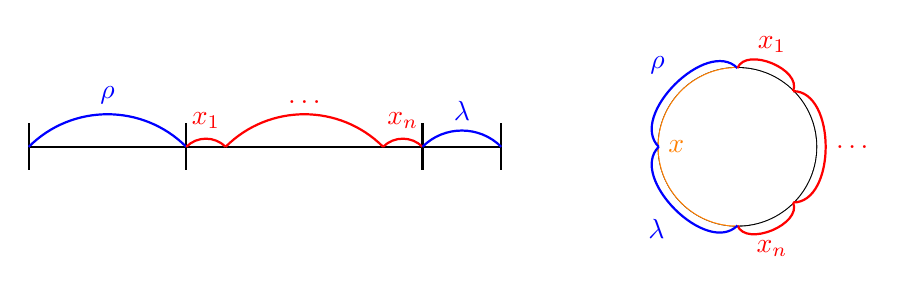
\begin{tikzpicture}
    \def \r {1}
    \coordinate (A) at (-9,0);
    \coordinate (B) at (-7,0);
    \coordinate (C) at (-4,0);
    \coordinate (D) at (-3,0);

    \draw[thick] (A) -- (D);
    \draw[thick] (A) -- ++(0,-0.3);
    \draw[thick] (A) -- ++(0,0.3);
    \draw[thick] (B) -- ++(0,-0.3);
    \draw[thick] (B) -- ++(0,0.3);
    \draw[thick] (C) -- ++(0,-0.3);
    \draw[thick] (C) -- ++(0,0.3);
    \draw[thick] (D) -- ++(0,-0.3);
    \draw[thick] (D) -- ++(0,0.3);

    \draw[thick,blue, bend left = 45] (A) to node[midway, above, blue]{\(\rho\)} (B);
    \draw[thick,red, bend left = 45] (B) to node[midway, above, red]{\(x_1\)} (-6.5,0);
    \draw[thick,red, bend left = 45] (-6.5,0) to node[midway, above, red]{\(\ldots\)} (-4.5,0);
    \draw[thick,red, bend left = 45] (-4.5,0) to node[midway, above, red]{\(x_n\)} (C);
    \draw[thick,blue, bend left = 45] (C) to node[midway, above, blue]{\(\lambda\)} (D);
    

    \draw[thick] (0,0) circle (\r);
    \draw[thick,orange] (0,-\r) arc[start angle=270, end angle=90, radius=\r] -- cycle;
    \fill[white] (0,0) circle (\r);
    \node[anchor=west, orange] at (-\r,0) {\(x\)};
    \draw[thick,blue, bend left = 90] (-\r,0) to node[midway, above left, blue]{\(\rho\)} (0,\r);
    \draw[thick,red, bend left = 90] (0,\r) to node[midway, above, red]{\(x_1\)} ({cos(45)},{sin(45)});
    \draw[thick,red, bend left = 90] ({cos(45)},{sin(45)}) to node[midway, right, red]{\(\ldots\)}({cos(-45)},{sin(-45)});
    \draw[thick,red, bend left = 90] ({cos(-45)},{sin(-45)}) to node[midway, below, red]{\(x_n\)} (0,-\r);
    \draw[thick,blue, bend left = 90] (0,-\r) to node[midway, below left, blue]{\(\lambda\)} (-\r,0);
    
  \end{tikzpicture}
  \caption{Rappresentazione grafica della definizione di codice circolare}\label{fig:circular_factorization}
\end{figure}

\begin{example}{}
  Il codice \(X = \set{ab,ba,bb}\) non è circolare. Considerando infatti la parola \(abab\). Si ha che, fissando \(\rho = a, \lambda = b\) che \(\lambda\rho = ba \in X\) e che \(\rho ba \lambda = abab \in \set{\rho}X^*\set{\lambda}\).
  Passando alla fattorizzazione circolare, è possibile ottenre \(abab\) nei seguenti modi:
  \begin{figure}[H]
    \centering
    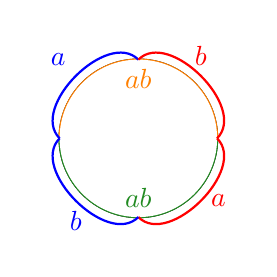
\begin{tikzpicture}
      \def \r {1}
      \draw[thick] (0,0) circle (\r);
      \draw[thick,orange] (-\r,0) arc[start angle=180, end angle=0, radius=\r] -- cycle;
      \draw[thick,ForestGreen] (-\r,0) arc[start angle=180, end angle=360, radius=\r] -- cycle;
      \fill[white] (0,0) circle (\r);
      \node[anchor=north, orange] at (0,\r) {\(ab\)};
      \node[anchor=south, ForestGreen] at (0,-\r) {\(ab\)};
      \draw[thick,blue, bend left = 90] (-\r,0) to node[midway, above left, blue]{\(a\)} (0,\r);
      \draw[thick,red, bend left = 90] (0,\r) to node[midway, above, red]{\(b\)} (\r,0);
      \draw[thick,red, bend left = 90] (\r,0) to node[midway, right, red]{\(a\)}(0,-\r);
      \draw[thick,blue, bend left = 90] (0,-\r) to node[midway, below, blue]{\(b\)} (-\r,0);
    
    \end{tikzpicture}
    \hspace{2cm}
    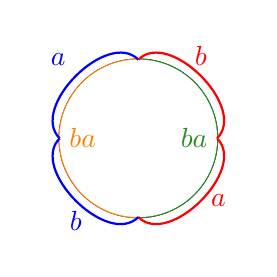
\begin{tikzpicture}
      \def \r {1}
      \draw[thick] (0,0) circle (\r);
      \draw[thick,orange] (0,-\r) arc[start angle=270, end angle=90, radius=\r] -- cycle;
      \draw[thick,ForestGreen] (0,-\r) arc[start angle=-90, end angle=90, radius=\r] -- cycle;
      \fill[white] (0,0) circle (\r);
      \node[anchor=west, orange] at (-\r, 0) {\(ba\)};
      \node[anchor=east, ForestGreen] at (\r,0) {\(ba\)};
      \draw[thick,blue, bend left = 90] (-\r,0) to node[midway, above left, blue]{\(a\)} (0,\r);
      \draw[thick,red, bend left = 90] (0,\r) to node[midway, above, red]{\(b\)} (\r,0);
      \draw[thick,red, bend left = 90] (\r,0) to node[midway, right, red]{\(a\)}(0,-\r);
      \draw[thick,blue, bend left = 90] (0,-\r) to node[midway, below, blue]{\(b\)} (-\r,0);
    
    \end{tikzpicture}
    \caption{Rappresentazione grafica della definizione di codice circolare}
  \end{figure}
  Inoltre, qualsiasi codice che contenga una parola che è potenza di una lettera non può essere circolare.
  Questo si può banalmente vedere considerando il caso in cui \(a^n \in X\) con \(a \in A\). Si ha necessariamente che \(a^{2n} = a^{\frac{n}{2}} a^n a^{\frac{n}{2}} \in X^*\) e dunque la fattorizzazione non è circolarmente univoca.
\end{example}

\begin{proposition}{Chi troppo vuole...}
  Sia \(X\) codice su \(A\) finito, circolare e massimale. Allora \(X = A\).
\end{proposition}

\begin{proof}
  Dal \Cref{cor:schutz_maximality_completeness} e dalla \Cref{prop:finite_complete_codes_contains_powers}, sappiamo che se \(X\) è massimale e finito, \(\forall a \in A, \exists n_a \geq 1 \st a^{n_a} \in X\)
  Poiché \(X\) è circolare, \(\forall a, n_a = 1\).
  Dunque \(A \subseteq X \implies X = A\), essendo \(A\) codice massimale su \(A^*\)
\end{proof}

\begin{theorem}{Restivo}
  Sia \(X\) codice su \(A\). Allora
  \begin{enumerate}
    \item \(X\) codice a ritardo di sincronizzazione finito \(\implies X\) circolare e a \keyword{parassitismo limitato}.
    \item \(X\) codice regolare, circolare e a parassitismo limitato \(\implies X\) codice a ritardo di sincronizzazione finito
  \end{enumerate}
\end{theorem}

\begin{note}{}
  Il parassitismo (limitato) non è stato trattato nel corso, poiché esula dagli argomenti principali.
  In maniera informale, un codice \(X\) ha parassitismo se esistono parole di \(X\) che contengono al loro interno parole di \(X^*\)
  Si parla di parassitismo limitato se esiste un limite superiore \(p\) alla lunghezza delle parole di \(X^*\) che possono essere contenute all'interno di parole di \(X\).
  Più formalmente,
  \[X \text{ ha parassitismo} \iff (A^+X^* A^*\cup A^*X^*A^+) \cap X \neq \emptyset\]
  \[X \text{ ha parassitismo limitato} \iff \exists p > 1 \st A^*X^p A^* \cap X = \emptyset\]

  Ciò che è d'interesse per questo corso, è che qualsiasi codice finito ha necessariamente parassitismo limitato.
\end{note}

\begin{corollary}{}
  Sia \(X\) codice finito, allora \(X\) codice a ritardo di sincronizzazione finito \(\iff X\) circolare.
\end{corollary}

\begin{corollary}{}
  Un codice a ritardo di sincronizzazione finito, binario e adattato a una sorgente propria \textbf{non} è ottimale (a meno che \(\# \SCal = 2\)).
\end{corollary}

\begin{proof}
  Dal corollario precedente, un codice a ritardo di sincronizzazione finito e adattato a una sorgente propria è circolare.
  Sappiamo inoltre che un codice binario ottimale è anche massimale.
  Dunque, per la proposizione precedente, l'unico codice finito binario circolare ottimale è l'alfabeto stesso, che però non è adattato a una sorgente propria con più di due simboli.
\end{proof}

\begin{definition}{Insiemi resto modificati}
  Sia \(X\) codice su \(A\). Definiamo l'insieme dei \keyword{resti modificati} di \(X\) come
  \begin{equation*}
    R_n'(X) = \begin{cases}
    Suff(X)\setminus (X \cup \set{\varepsilon}) & n = 1\\
    {R_{n-1}'(X)}^{-1}X \cup X^{-1}R_{n-1}'(X) & n > 1
    \end{cases}
  \end{equation*}
\end{definition}

\begin{theorem}{Levenshtein}
  \(X\) circolare \(\iff \exists n \geq 1 \st R_n'(X) = \emptyset\)
\end{theorem}

\begin{observation}{}
  Per \(X\) codice (finito),
  \[R_1 = X^{-1}X\setminus \set{\varepsilon} \subseteq Suff(X) \setminus (X \cup \set{\varepsilon}) = R_1' \implies \forall n \geq 1, R_n \subseteq R_n'\]
  Questo è un altro modo per dimostrare che se \(X\) ha ritardo di sincronizzazione finito, allora ha ritardo di decifrazione finito.
  Infatti se ha ritardo di sincronizzazione finito, allora ha \(R_n' = \emptyset\) per qualche \(n\), dunque anche \(R_n = \emptyset\) per lo stesso \(n\), e quindi ha ritardo di decifrazione finito per teoremi visti prima 
\end{observation}

\begin{example}{}
  \(X = \set{a,ba,bb}\) \textbf{non} è circolare.
  Infatti \(R_1' = Suff(X) \setminus (X \cup \set{\varepsilon}) = \set{b}\).
  Inoltre \(R_2' = {R_1'}^{-1}X \cup X^{-1}R_1' = \set{a,b}\).
  \(R_3' = \set{\varepsilon, a ,b}\),\(R_4' = \set{\varepsilon, a ,b, ba,bb} = R_n' \forall n \geq 4\).

  Invece \(X' = \set{ab,aab}\) circolare: \(R_1' = \set{b}, R'_2 = \emptyset\)
  Anche \(X'' = \set{ab,aba,ba^3,b^2a}\) è circolare:
  \(R_1' = \set{a,b,a^2,ba,a^3}, R_2' = \set{b,ba,a^3,a^2}, R_3' = \set{a^3,ba,a^3}, R_4' = \set{a^3}, R_5' = \emptyset\)
\end{example}

